% 2003 年全国新课程理科第 15 题：花圃着色图
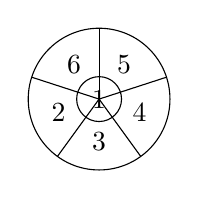
\begin{tikzpicture}[scale=0.75]
  \draw (0,0) circle (1.2);
  \foreach \angle in {90,18,-54,-126,162}
    \draw (0,0)--(\angle:1.2);
  \draw (0,0) circle (0.38);
  \node at (0,0) {1};
  \node at (54:0.72) {5};
  \node at (-18:0.72) {4};
  \node at (-90:0.72) {3};
  \node at (-162:0.72) {2};
  \node at (126:0.72) {6};
\end{tikzpicture}
